\section{Diskussion}
\label{sec:Diskussion}
Die Differenz zwischen dem berechneten $R_\text{eff}$ und dem in der Schaltung eingebauten Widerstand $R_\text{1}$ beträgt$\Delta R=60.1 \,\si{\ohm}$.
Diese lässt sich auf Innenwiderstand des Funktionengenerators von $R=50\,\si{\ohm}$ zurückführen.
Daher wird, wie in der Auswertung erwähnt, der Generatorinnenwiderstand in den Berechnungen berücksichtigt.
Die verbleibende Differenz lässt sich mit kleinen Messunsicherheiten -- also statistischen Fehlern -- begründen und liegt annähernd im Toleranzbereich.

Bei der Bestimmung des Dämpfungswiderstandes $R_{\mathrm{ap}}$ zeigt sich eine Abweichung 
des experimentell bestimmten Wertes von $29\%$ zum Theoriewert. Dies lässt sich einerseits 
auf das Vernachlässigen von den Innenwiderständen der weiteren Bauteile zurückführen und 
andererseits auf Schwierigkeiten beim Ablesen des Widerstandes. Im Grenzbereich zeigten 
sich keine erkennbaren Unterschiede der Kondensatorspannung. 

Beim Vergleich der gemessenen beziehungsweise aus den Plots abgelesenen Messgrößen zeigen sich nur geringe Abweichungen gegenüber den Theoriewerten.
Im Detail zeigt ein Vergleich zwischen der theoretisch aus den Kenngrößen des Schwingkreises berechneten Güte $q_\mathrm{Theorie}$ mit der experimentell bestimmten Güte $q_\mathrm{Experiment}$ eine Abweichung von $8\%$.
Für die Breite der Resonanzkurve ergibt sich eine Abweichung von $5\%$.

Für die bestimmten Werte bei der Beobachtung der Phasenverschiebung in Abhängigkeit von der 
Frequenz zeigt sich für $\omega_1$ und $\omega_{\mathrm{res}}$ eine Abweichung kleiner als $1\%$. Für $\omega_2$ erhält man selbige zu $4\%$.

Die abgelesenen Werte liegen alle absolut im Rahmen der Toleranz und sind auf statistische Fehler 
und Ablesefehler zurückzuführen.

Allerdings fiel bereils zu Beginn der Messung auf, dass der Funktionengenerator keinen richtigen Nadelimpuls lieferte. Stattdessen lieferte der Generator einen Rechteckimpuls. Vergleiche dazu Abbildung \ref{fig:blabliblub}.
Wahrscheinlich wird dies allerdings wenig Einfluss auf die Messung gehabt haben.

\begin{figure}
	\centering
	\caption{Spannungsverlauf der Generatorspannung bei eingestellter Nadelimpulsfunktion.}
	\label{fig:blabliblub}
	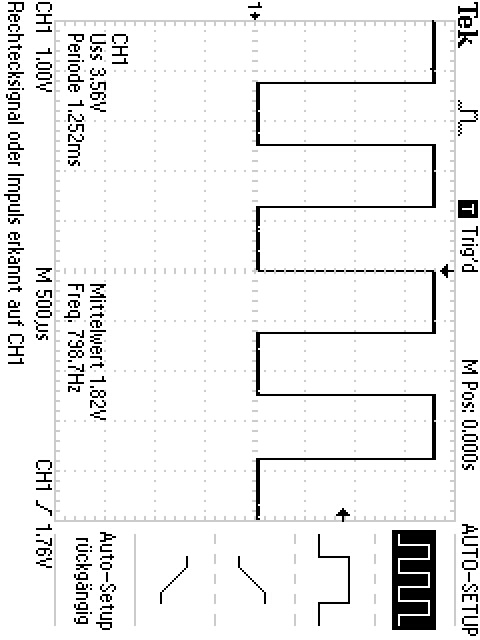
\includegraphics[width = 0.6 \textwidth, angle=90]{Bilder/a)rectangle/F0001TEK.JPG}
\end{figure}
